% Toolbar icon: saveAs — a floppy disk with a pencil overlaid (save to a new file).
\documentclass[tikz,border=2mm]{standalone}
\usetikzlibrary{arrows.meta,calc,shapes.geometric}
\begin{document}
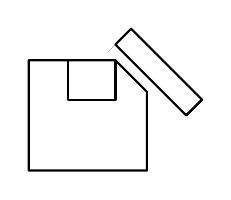
\begin{tikzpicture}[line width=1.3pt, line cap=round, line join=round, >=Stealth, x=1mm,y=1mm]
  % floppy disk (kept to the lower-left to leave room for the pencil)
  \draw[thick] (-10,-9) -- (-10,5) -- (1,5) -- (5,1) -- (5,-9) -- cycle;
  \draw[thick] (-5,5) -- (-5,0) -- (1,0) -- (1,5);
  % pencil across the top-right
  \draw[thick] (1,7) -- (3,9) -- (12,0) -- (10,-2) -- cycle;
  \draw[thick] (10,-2) -- (12,0);
  \fill (0,6) -- (1,7) -- (3,9) -- (2,8) -- cycle;
\end{tikzpicture}
\end{document}
